\documentclass[12pt,fleqn]{article}\usepackage{../../common}
\begin{document}
Sonlu Öğeler Metotu (Finite Elements Method -FEM-) - 2

Önceki örnekler standart eni değişmeyen kiriş yapısını temel aldı.  Fakat ya
kiriş alttaki gibi olsaydı?

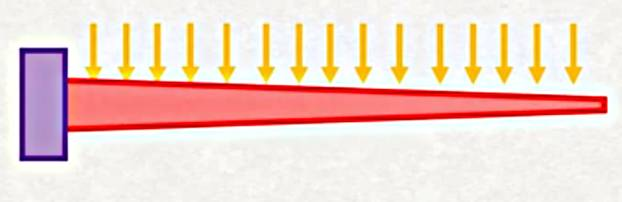
\includegraphics[width=15em]{compscieng_bpp45fem2_01.jpg}

Bu kirişi temsilen

$$
E I \frac{\ud^4 y}{\ud X_1^4} = q
$$

diferansiyel denklemini hala kullanabilir miyiz? Dikkat edersek en değiştiğine
göre $X_1$ ile beraber, ona bağlı olarak, atalet momenti $I$ sabit değil,
değişken demektir.. Bazıları düşünebilir ``ama o zaman değişken $I$'yi alırız,
üstteki denklemdeki $I$'ya sokarız olur biter''. Bunu yapamayız çünkü $I$'nin
sabit olması üstteki denklemi türetmek için bir önkabuldu, yani $I$ değişken ise
üstteki denklemi kullammak mümkün değildir [1, Ders 4].

Problem şu ki pek çok gerçek dünya uygulaması üstteki Euler-Bernoulli kiriş
formülüne erişirken kullandığımız faraziyelere uymaz, bunları hatırlarsak lineer
elastiklik, yok sayılabilecek Poisson etkileri, düzlemlerin düz kalması idi.
Fakat mesela beton materyelini ele alalım, bu materyel ucuzdur, basınca, yani
içe doğru strese karşı çok dayanıklıdır, ki bu yüzden pek çok yapıda kullanılır,
fakat beton dışa doğru stres, yani gerilime karşı dayanıklı değildir. Çok az bir
yükü bile beton parçaya dışa doğru uygulasam çatlamaya başlar, çatlamak demek
oradaki yüzeyin bozulmaya uğraması demektir, ki dolaylı olarak $I$
değisecektir. Diğer bir problem yüke bağlı olarak betonun $E$ değerinin de
değişmesi. Yani gerçek dünyada $I$ neredeyse hiçbir zaman sabit değildir, $E$
benzer şekilde, durumu daha kötü yapan bu değişimlerin çoğunlukla yük $q$
değerine bağlı olması. Bu herşeyi arap saçına döndürür.

Problemin çözümü FEM yaklaşımında. Nasıl? Çünkü eğer bir kirişi yeterince ufak
parçalara bölebilirsem o parçalarda $I$, ve $E$ sabit kabul edebilirim ve bu
parçalarda daha basit olan denklemleri kullanabilirim. FEM matematiği bana bu
parçaları birleştirmem için güzel bir mekanizma sağlıyor zaten.

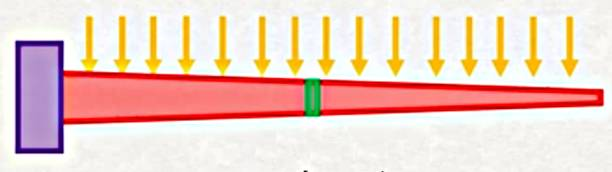
\includegraphics[width=15em]{compscieng_bpp45fem2_02.jpg}

Üstteki resimdeki yeşil bölgeyi düşünelim, o bölgenin iki yan yüzeylerini
düşünürsek, belki soldan sağa giderken biraz değişim olur ama parça çok ufak
olduğu için bu değişim fazla değildir. 

FEM maceramıza çubuk/makaskiriş (bar/truss) öğeleri ile devam edeceğiz.  Bu
yapılar çok basit olmalarına rağmen FEM metadolojisini göstermesi açısından çok
uygunlar. Onları sadece küçülme, esneme açısından inceleyeceğiz, moment,
kaykılma gibi konuları şimdilik yok sayacağız. Fakat işleyeceğimiz pek çok
yaklaşım, ``dırengenlikleri (stiffness)'' hesaplarken kullandığımız adımlar her
FEM hesabında faydalı olan kavramlar.





















[devam edecek]

[1] Petitt, {\em Intro to the Finite Element Method}, University of Alberta,
    \url{https://www.youtube.com/watch?v=2iUnfPRk6Ro&list=PLLSzlda_AXa3yQEJAb5JcmsVDy9i9K_fi}

\end{document}
